%-------------------------------------------------------------------------------
%	CAPITOLO 37
%-------------------------------------------------------------------------------

\chapter{Un telegramma}
Il buon \index[Personaggi]{M. P.}P. M. aveva un figlio all'università, con tutte le preoccupazioni della spesa da sostenere e delle bagatelle che esso figlio gli poteva procurare per la sua gioventù e vivacità.\\
\indent Un giorno il signor \index[Personaggi]{M. P.}P.\:.\:.\: si vide recapitare un telegramma, vergato a grossi caratteri dal collettore locale postegrafico \index[Personaggi]{Mercatelli (collettore postale)}Barandellaccio di Mercatelli, così:\\ \textcal \Huge\\
\centerline {Vostro figlio carcerato}\\
\centerline {firmato da persona amica}\\ \normalfont \normalsize \\
\indent Il povero uomo, cominciò a disperarsi, in fretta e furia riempire il portafoglio, perché in qualunque disgrazia bisogna cominciare a vuotarlo... attacca il cavallo e via a \index[Luoghi]{Lugo}Lugo per prendere il treno per \index[Luoghi]{Bologna}Bologna.\\
\indent Il lettore potrà bene immaginare i tristi pensieri che accompagnavano il nostro uomo fino a \index[Luoghi]{Bologna}Bologna... dove arrivò più morto che vivo.\\
\indent Appena arrivato a Bologna, trafilato si recò all'abitazione del figlio e trovata la padrona di casa subito l'apostrofò: <<Mio figlio?>>\\
\indent Padrona: <<È fuori in baldoria con gli amici.>>\\
\indent \index[Personaggi]{M. P.}P.\:.\:.\: : <<Oh, mio signore ma che cos'ha fatto che l'hanno arrestato?>>\\
\indent Padrona: <<Arrestato! Non so nulla. Andiamo a vedere in trattoria.>>\\
\indent In trattoria trovarono un'orgia infernale a banchetto di studenti e non c'era caso né di parlare, né di farsi ascoltare.\\
\indent Con un pò di pazienza trovarono il sospirato figlio... laureato... e la scena cambiò... con una smunta allegra e simpatica al portafoglio di papà.\\
\indent Quel \index[Personaggi]{Mercatelli (collettore postale)}Barandellaccio del telegrafo ne combinava delle curiose!

\vspace{1cm}
\centerline{\rule{1.5cm}{0.4pt}}
\vspace{1cm}

\begin{figure}[htb]
    \centering
    %\vspace{-0.7cm}
    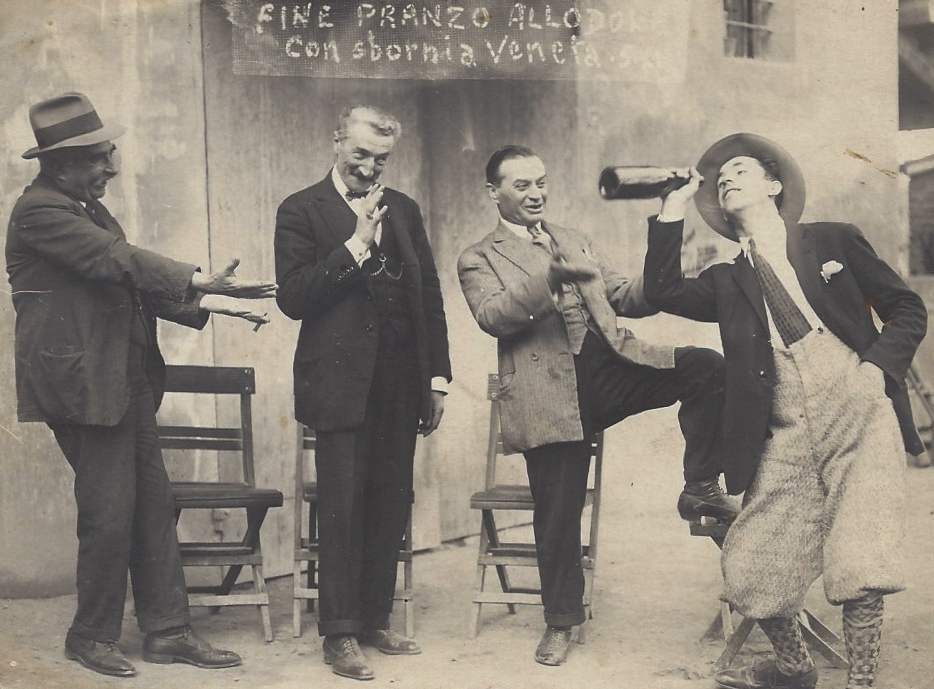
\includegraphics[width=\textwidth]{sbornia}
    \caption[Bevitori - "Sbornia Veneta"]{Una simpatica fotografia trovata nell'archivio di Mingazzi. "Fine Pranzo Allodole - Sbornia Veneta - 5 XI". Da sinistra: Dr.\:Cassiano Meruzzi \index[Personaggi]{Meruzzi dott. Cassiano}, \index[Personaggi]{Tazzari Luciano (fotografo)}Luciano Tazzari (fotografo), Nando Isani\index[Personaggi]{Isani Nando}, Dr.\:Domenico Stella\index[Personaggi]{Stella dott. Domenico}. \label{fig:sbornia}}
    %\vspace{-0.3cm}
\end{figure}